% options:
% thesis=B bachelor's thesis
% thesis=M master's thesis
% czech thesis in Czech language
% slovak thesis in Slovak language
% english thesis in English language
% hidelinks remove colour boxes around hyperlinks
% 10pt 11pt 12pt

\documentclass[thesis=M,slovak]{FITthesis}[2013/05/06]

\usepackage[utf8]{inputenc} % LaTeX source encoded as UTF-8

\usepackage{graphicx} %graphics files inclusion
\usepackage{hyperref} %hypertext
\usepackage{graphicx}
% \usepackage{amsmath} %advanced maths
% \usepackage{amssymb} %additional math symbols

\usepackage{dirtree} %directory tree visualisation

% % list of acronyms
% \usepackage[acronym,nonumberlist,toc,numberedsection=autolabel]{glossaries}
% \iflanguage{czech}{\renewcommand*{\acronymname}{Seznam pou{\v z}it{\' y}ch zkratek}}{}
% \makeglossaries

\newcommand{\tg}{\mathop{\mathrm{tg}}} %cesky tangens
\newcommand{\cotg}{\mathop{\mathrm{cotg}}} %cesky cotangens

% % % % % % % % % % % % % % % % % % % % % % % % % % % % % % 
% ODTIALTO DALEJ VSETKO ZMENTE
% % % % % % % % % % % % % % % % % % % % % % % % % % % % % % 

\department{Katedra \ldots (DOPLŇTE)}
\title{Doplňte názov práce}
\authorGN{Doplňte Vaše krstné meno/mená} %(krstné) meno (mená) autora
\authorFN{Doplňte Vaše priezvisko} % priezvisko autora
\authorWithDegrees{Doplňte Vaše meno a tituly} %meno autora včetne súčasných akademických titulov
\supervisor{Doplňte meno vedúceho práce}
\acknowledgements{Doplňte, ak chcete niekomu za niečo poďakovať. V~opačnom prípade úplne odstráňte tento príkaz.}
\abstractCS{V niekoľkých vetách zhrňte obsah a prínos tejto práce v~slovenčine. Po prečítaní abstraktu by mal čitateľ mať dosť informácií pre rozhodnutie, či Vašu prácu chce čítať.}
\abstractEN{Sem doplňte ekvivalent abstraktu Vašej práce v~angličtině.}
\placeForDeclarationOfAuthenticity{V~Prahe}
\declarationOfAuthenticityOption{1} %voľba Prehlásenia (číslo 1-6)
\keywordsCS{Nahraďte zoznamom kľúčových slov v slovenčine oddelených čiarkou.}
\keywordsEN{Nahraďte zoznamom kľúčových slov v angličtine oddelených čiarkou.}
% \website{http://site.example/thesis} %volitelná URL práce, objeví se v tiráži

\begin{document}

% \newacronym{CVUT}{{\v C}VUT}{{\v C}esk{\' e} vysok{\' e} u{\v c}en{\' i} technick{\' e} v Praze}
% \newacronym{FIT}{FIT}{Fakulta informa{\v c}n{\' i}ch technologi{\' i}}

\begin{introduction}
	%sem napíšte úvod Vašej práce
\end{introduction}

\chapter{Popis problému}
Repozitár slúži vo všeobecnosti ako centrálne miesto, ktoré sa stará o ukladanie a správu dát. Takúto službu môžu chcieť poskytovať rôzne inštitúcie (napríklad školy), knihovny,... Pod slovom repozitár si môžeme taktiež predstaviť konkrétny software, ktorý sa stará o ukladanie, archiváciu a sprístupnenie dát. V tejto diplomovej práci budeme pod slovom repozitár rozumieť práve software.

\section{Zdieľanie dát v teame}
Ústav organickej chémie VŠCHT Praha potrebuje vyriešiť ukladanie a sprístupnenie dát. Potrebujú ukladať, analyzovať a prezentovať infračervené vibračné, NMR a hmotnostné spektroskopické merania, chemické vzorce a reakcie.

Nad jedným datasetom môže pracovať viacero ľudí, ktorý môžu riešiť rôzne merania a pokusy alebo spoločne pracovať na jednom meraní. V oboch prípadoch, počas priebehu samotného výskumu, potrebujú prístup k dátam, ktoré vytvoril iný člen teamu. Taktiež musia mať možnosť dáta upravovať (napr. opakované merania a pokusy, keď je potrebné doplniť nové výsledky). Je teda potrebné vyriešiť zdieľanie dát v teame, rôzne oprávnenia pre osoby, ktoré majú mať k dátam prístup, verzovanie dát.

\section{Open data/Open access}
Taktiež je pri vývoji repozitára potrebné myslieť na možnosť zverejnenia (časti) dát pre širokú verejnosť s možnosťou ich ďalšieho využitia alebo odkazovania sa na ne. Takto zverejnené dáta označujeme pojmom Open data. V prípade zverejnených výzkumov hovoríme o Open access (OA).

\section{Zálohovanie a archivácia}
Zálohovaním dát rozumieme vytváranie kópie práve spracúvaných alebo v relatívne nedávnej dobe uložených dát. Archiváciou rozumieme uschovávanie dokumentačných materiálov.

Zálohované dáta môžu byť poškodené degradáciou média, fyzickým poškodením média alebo v súčasnosti rozšírenými cryptovírusmi. Zálohovať dáta na jedno médium nestačí. Je dobré sa riadiť pravidlom 3-2-1. Tri kópie všetkých dôležitých dát, na dvoch rôznych médiach, pričom jedna kópia by mala byť uložená off-site, teda niekde mimo pracovného prostredia. \cite{zalohovanie}

Pri archivácii dát je potrebné myslieť na čitateľnosť dát po dlhej dobe. Preto je potrebné myslieť nie len na zabezpečenie dát, ale aj na archiváciu programu potrebného pre prečítanie archivovaných dát.

Repozitár by mal byť pre užívateľov možnosťou ako dáta zálohovať. Zároveň jeho napojenie na služby CESNETu umožní ochranu dát, akú by bolo na pracovisku VŠCHT Praha ťažké dosiahnúť.

V budúcnosti bude možné repozitár rozšíriť o nástroje, ktoré by umožnili aj dlhodobú archiváciu dát.

\chapter{Súčasné riešenia}
\section{Bežné repozitáre}
Existujú rôzne repozitáre, ktoré sa od seba líšia použitou technológiou, možnosťou rozšírenia, používajú rôzne metadátové schémy. Niektoré sú voľné dostupné ako open source iné ako proprietárny software alebo hosťované aplikácie. V tejto časti je prehľad dostupných aplikácií. Zameriavam sa najmä na vlastnosti, ktoré boli pre ďalší vývoj repozitára kľúčové a to: open source (aby bolo možné software ďalej upravovať), použitie metadátovej schémy, modulárnosť softwaru (jednoduchá možnosť rozšírenia o ďalšie nástroje) a verzovanie (najmä kvôli zdieľaniu a zálohovaniu dát).

% Tento software sa zameriava na dokumenty, ktoré majú byť voľne dostupné (anglicky Open Access) a online. Najčastejšie sa do takýchto inštitucionálnych repozitárov ukladajú textové dokumenty, pre ktoré je software najlepšie prispôsobený.

\subsection{Metadáta}
Na popis uložených dokumentov slúžia metadáta. Metadáta sú štrukturované dáta nesúce informáciu o primárnych dátach.\cite{iso8459-5} Kvôli vzájomnej prepojenosti repozitárov, vyhľadávaní dát a správnej interpretácii informácií je snaha o vyvinutie celosvetovo používaného štandardu pre popis dát.

O to sa snažia rôzne metadátove schémy, pomocou ktorýchi je možné zdroje popísať. Medzi najznámejšie schémy patrí Dublin Core [\url{http://dublincore.org/}] a MARC [\url{http://www.loc.gov/marc/}].


Dublin Core (skrátene DC) vznikol s cieľom jednoducho a všeobecne popísať webové zdroje. Táto schéma obsahuje 15  prvkov. To sú: názov (title), autor (creator), predmet (subject), popis (description), vydavateľ (publisher), prispievateľ (contributor), dátum (date), typ (type), formát (format), identifikátor (identifier), zdroj (source), jazyk (language), vzťah (relation), pokrytie (coverage) a práva (rights). Tieto prvky nie sú povinné a môžu sa opakovať. Jednotlivé vlastnosti sú teda pomenované. Ako sa World Wide Web menil, v snahe o vytvorenie sémantického webu, sa vyvinul aj štandard Dublin Core. Od roku 2008 obsahuje formálne domény a rozsahy v definiciách vlastností. Táto aktualizovaná varianta vlastností sa nazýva dcterms. Jednotlivé prvky môžu ďalej obsahovať kvalifikátor. Ten môže lepšie určiť, čo daná položka popisuje. Napríklad namiesto všeobecného autora tak môžeme upresniť, či išlo o ilustrátora (dc:creator.ilustrator), editora (dc:creator.editor),...  Pre systémy, ktoré kvalifikátory nepoužívajú ale musí zostať význam zachovaný.


MARC využívajú najmä knihovníci. Bol navrhnutý pre popis bibliografických údajov v strojovo čitateľnej podobe.
Schéma obsahuje vlastnosti, ktoré sú očíslované. Kým názov v dcterms je označený ako title, v MARCu  je označený číslom 245 (title proper statement). Na rozdiel od dcterms obsahuje niekoľko pomocných polí (ako napríklad 222 kľúčový názov, 240 unifikovaný názov,...). 

\subsection{Software}

\subsubsection {Digital Commons}  [\url{http://digitalcommons.bepress.com/}]

Hostovaná platforma inštitucionálneho repozitára. Zameraný na školy a školské dokumenty.

Používa Dublin Core schému, v používateľskom rozhraní podporuje aj iné vlastnosti než len DC, aj keď nepodporuje iné schémy (vrátane MARC).

Autori vedia prispôsobiť repozitár požiadavkám klienta.

Nepodporuje verzovanie.

\subsubsection {LIBSYS}  [\url{http://www.libsys.co.in/}]

Proprietárny software. Repozitár funguje ako webová aplikácia.

Používa MARC ako schému metadát.

\subsubsection {SimpleDL}  [\url{http://www.simpledl.com/}]

Proprietárny software.

Metadáta na základe Dublin Core. Môžu byť rozšírené o iné schémy.

\subsubsection {Greenstone}  [\url{http://www.greenstone.org/}]

Repozitár vyvinutý na Univerzite Waikato.

Používa MARC schému.

Modulárna architektúra, napísaný v jazyku Java. Pluginy v jazyku Perl.

Nepodporuje verzovanie.

Open source

\subsubsection {Invenio}  [\url{http://inveniosoftware.org/}]

Software bol pôvodne vyvinutý pre CERN. Umožňuje vytvoriť digitálnu knihovňu alebo repozitár dokumentov dostupný cez web. 

Používa špecifikáciu MARC pre metadáta.

Má modulárnu architektúru. Napísaný v jazyku Python.

Podporuje verzovanie uložených dát.

Open Source

\subsubsection {Zenodo} [\url{https://zenodo.org/}]

Vyvinutý na základe Invenia, taktiež pre CERN. Má teda rovnaké vlastnosti ako Invenio.

\subsubsection {EPrints} [\url{http://www.eprints.org/}]

Vyvinutý na Univerzite Southampton.

Používa rôzne typy metadátových polí, ktoré je možné nastavovať (upraviť zobrazovanie, indexovanie, vyhľadávanie).

Modulárny software napísaný v jazyku Perl.

Podporuje verzovanie dát.

Open Source

\subsubsection {DSpace} [\url{http://www.dspace.org/}]

Software pôvodne vyvinutý MIT a Hewlett-Packard. Od vzniku má viac ako 2000 inštalácií po celom svete. 

Ako východziu schému pre popis dát používa Dublin Core, je však možné použiť aj iné schémy.

Ide o súbor spolupracujúcich Java webových aplikácií. K dispozícií je RESTful webové užívateľské rozhranie.

Neumožňuje verzovanie uložených dát.

Open source

\subsubsection {Fedora} [\url{http://www.fedora-commons.org/}]

Je možné použiť rôzne schémy pre popis dát.

Flexibilný, jednoducho rozšíriteľný, modulárny repozitár. Napísaný v programovacom jazyku Java.

Umožňuje verzovanie uložených dát.

Open Source


\quad

Vrámci diplomovej práce pracujem s Fedorou verzie 4.5.
Kvôli požiadavkom, ktoré sú kladené na repozitár, budeme potrebovať upraviť fungovanie REST frameworku. A to tak, aby aplikácia kontrolovala oprávnenia na zmenu stavov už pri spracovaní požiadavku.

Nad RESTapi bude postavené užívateľské webové rozhranie. Napájať sa teda budeme na vrstvu, ktorá sa stará o prístup k dátam a ich uchovávanie.

%\begin{figure}[h]
%\centering
%\caption{Architektúra komponentov \url{https://wiki.duraspace.org/display/FEDORA45/Fedora+4.5+Documentation}}
%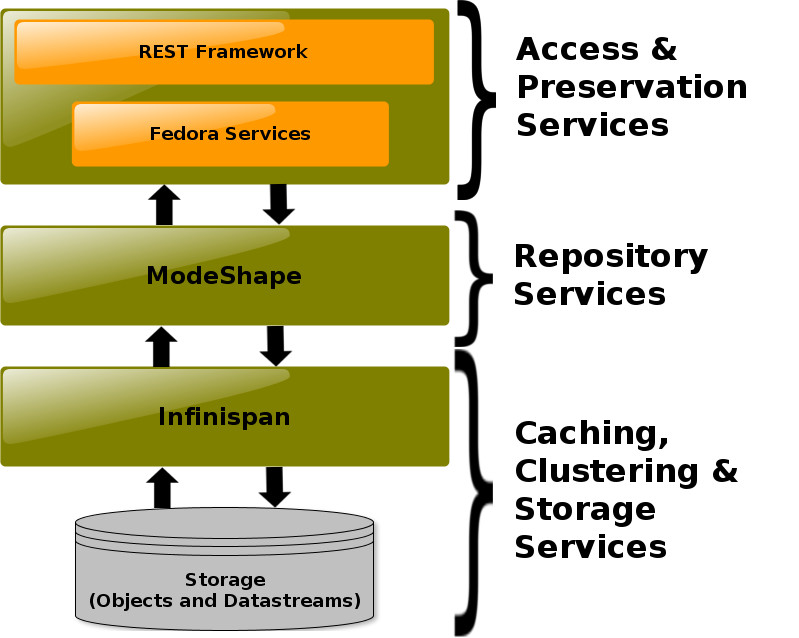
\includegraphics[width=1.0\textwidth]{f4-stack.jpg}
%\end{figure}
%
%
%\begin{figure}[h]
%\centering
%\caption{Integrácia komponentov \url{https://wiki.duraspace.org/display/FEDORA45/Fedora+4.5+Documentation}}
%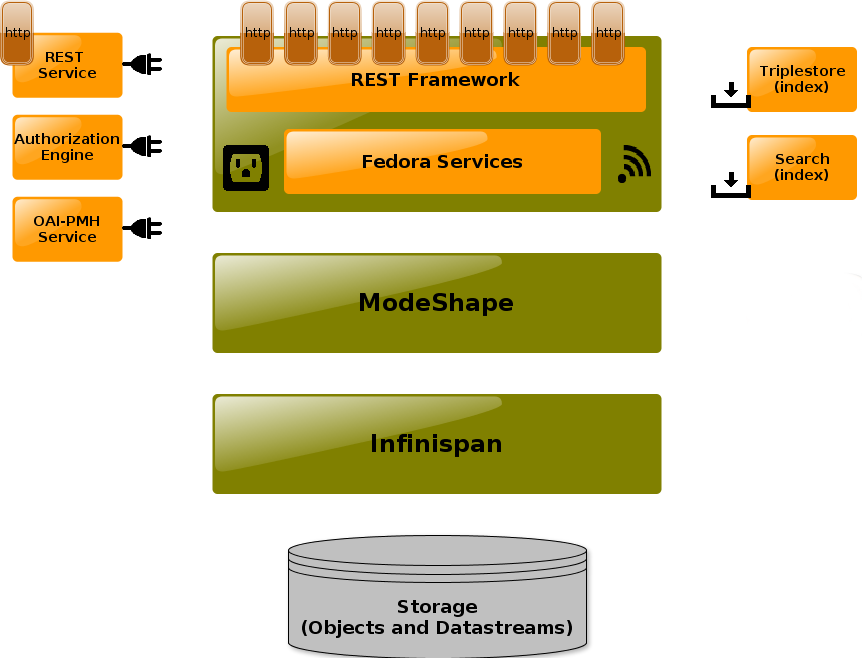
\includegraphics[width=1.0\textwidth]{f4-arch.png}
%\end{figure}
%
%
%Systémove požiadavky:
%\begin{enumerate}
%	\item Java 8
%	\item Servlet 3.0 container (Tomcat 7 a novší, Jetty 9.x a novší...)
%\end{enumerate}


\chapter{Realizácia}

\begin{conclusion}
	%sem napíšte záver Vašej práce
\end{conclusion}

\bibliographystyle{csn690}
\bibliography{mybibliographyfile}

\appendix

\chapter{Zoznam použitých skratiek}
% \printglossaries
\begin{description}
	\item[GUI] Graphical user interface
	\item[XML] Extensible markup language
\end{description}


% % % % % % % % % % % % % % % % % % % % % % % % % % % % 
% % Tuto kapitolu z výsledné práce ODSTRAŇTE.
% % % % % % % % % % % % % % % % % % % % % % % % % % % % 
% 
% \chapter{Návod k~použití této šablony}
% 
% Tento dokument slouží jako základ pro napsání závěrečné práce na Fakultě informačních technologií ČVUT v~Praze.
% 
% \section{Výběr základu}
% 
% Vyberte si šablonu podle druhu práce (bakalářská, diplomová), jazyka (čeština, angličtina) a kódování (ASCII, \mbox{UTF-8}, \mbox{ISO-8859-2} neboli latin2 a nebo \mbox{Windows-1250}). 
% 
% V~české variantě naleznete šablony v~souborech pojmenovaných ve formátu práce\_kódování.tex. Typ může být:
% \begin{description}
% 	\item[BP] bakalářská práce,
% 	\item[DP] diplomová (magisterská) práce.
% \end{description}
% Kódování, ve kterém chcete psát, může být:
% \begin{description}
% 	\item[UTF-8] kódování Unicode,
% 	\item[ISO-8859-2] latin2,
% 	\item[Windows-1250] znaková sada 1250 Windows.
% \end{description}
% V~případě nejistoty ohledně kódování doporučujeme následující postup:
% \begin{enumerate}
% 	\item Otevřete šablony pro kódování UTF-8 v~editoru prostého textu, který chcete pro psaní práce použít -- pokud můžete texty s~diakritikou normálně přečíst, použijte tuto šablonu.
% 	\item V~opačném případě postupujte dále podle toho, jaký operační systém používáte:
% 	\begin{itemize}
% 		\item v~případě Windows použijte šablonu pro kódování \mbox{Windows-1250},
% 		\item jinak zkuste použít šablonu pro kódování \mbox{ISO-8859-2}.
% 	\end{itemize}
% \end{enumerate}
% 
% 
% V~anglické variantě jsou šablony pojmenované podle typu práce, možnosti jsou:
% \begin{description}
% 	\item[bachelors] bakalářská práce,
% 	\item[masters] diplomová (magisterská) práce.
% \end{description}
% 
% \section{Použití šablony}
% 
% Šablona je určena pro zpracování systémem \LaTeXe{}. Text je možné psát v~textovém editoru jako prostý text, lze však také využít specializovaný editor pro \LaTeX{}, např. Kile.
% 
% Pro získání tisknutelného výstupu z~takto vytvořeného souboru použijte příkaz \verb|pdflatex|, kterému předáte cestu k~souboru jako parametr. Vhodný editor pro \LaTeX{} toto udělá za Vás. \verb|pdfcslatex| ani \verb|cslatex| \emph{nebudou} s~těmito šablonami fungovat.
% 
% Více informací o~použití systému \LaTeX{} najdete např. v~\cite{wikilatex}.
% 
% \subsection{Typografie}
% 
% Při psaní dodržujte typografické konvence zvoleného jazyka. České \uv{uvozovky} zapisujte použitím příkazu \verb|\uv|, kterému v~parametru předáte text, jenž má být v~uvozovkách. Anglické otevírací uvozovky se v~\LaTeX{}u zadávají jako dva zpětné apostrofy, uzavírací uvozovky jako dva apostrofy. Často chybně uváděný symbol "{} (palce) nemá s~uvozovkami nic společného.
% 
% Dále je třeba zabránit zalomení řádky mezi některými slovy, v~češtině např. za jednopísmennými předložkami a spojkami (vyjma \uv{a}). To docílíte vložením pružné nezalomitelné mezery -- znakem \texttt{\textasciitilde}. V~tomto případě to není třeba dělat ručně, lze použít program \verb|vlna|.
% 
% Více o~typografii viz \cite{kobltypo}.
% 
% \subsection{Obrázky}
% 
% Pro umožnění vkládání obrázků je vhodné použít balíček \verb|graphicx|, samotné vložení se provede příkazem \verb|\includegraphics|. Takto je možné vkládat obrázky ve formátu PDF, PNG a JPEG jestliže používáte pdf\LaTeX{} nebo ve formátu EPS jestliže používáte \LaTeX{}. Doporučujeme preferovat vektorové obrázky před rastrovými (vyjma fotografií).
% 
% \subsubsection{Získání vhodného formátu}
% 
% Pro získání vektorových formátů PDF nebo EPS z~jiných lze použít některý z~vektorových grafických editorů. Pro převod rastrového obrázku na vektorový lze použít rasterizaci, kterou mnohé editory zvládají (např. Inkscape). Pro konverze lze použít též nástroje pro dávkové zpracování běžně dodávané s~\LaTeX{}em, např. \verb|epstopdf|.
% 
% \subsubsection{Plovoucí prostředí}
% 
% Příkazem \verb|\includegraphics| lze obrázky vkládat přímo, doporučujeme však použít plovoucí prostředí, konkrétně \verb|figure|. Například obrázek \ref{fig:float} byl vložen tímto způsobem. Vůbec přitom nevadí, když je obrázek umístěn jinde, než bylo původně zamýšleno -- je tomu tak hlavně kvůli dodržení typografických konvencí. Namísto vynucování konkrétní pozice obrázku doporučujeme používat odkazování z~textu (dvojice příkazů \verb|\label| a \verb|\ref|).
% 
% \begin{figure}\centering
% 	
\includegraphics[width=0.5\textwidth, angle=30]{cvut-logo-bw}
% 	\caption[Příklad obrázku]{Ukázkový obrázek v~plovoucím prostředí}\label{fig:float}
% \end{figure}
% 
% \subsubsection{Verze obrázků}
% 
% % Gnuplot BW i barevně
% Může se hodit mít více verzí stejného obrázku, např. pro barevný či černobílý tisk a nebo pro prezentaci. S~pomocí některých nástrojů na generování grafiky je to snadné.
% 
% Máte-li například graf vytvořený v programu Gnuplot, můžete jeho černobílou variantu (viz obr. \ref{fig:gnuplot-bw}) vytvořit parametrem \verb|monochrome dashed| příkazu \verb|set term|. Barevnou variantu (viz obr. \ref{fig:gnuplot-col}) vhodnou na prezentace lze vytvořit parametrem \verb|colour solid|.
% 
% \begin{figure}\centering
% 	\includegraphics{gnuplot-bw}
% 	\caption{Černobílá varianta obrázku generovaného programem Gnuplot}\label{fig:gnuplot-bw}
% \end{figure}
% 
% \begin{figure}\centering
% 	\includegraphics{gnuplot-col}
% 	\caption{Barevná varianta obrázku generovaného programem Gnuplot}\label{fig:gnuplot-col}
% \end{figure}
% 
% 
% \subsection{Tabulky}
% 
% Tabulky lze zadávat různě, např. v~prostředí \verb|tabular|, avšak pro jejich vkládání platí to samé, co pro obrázky -- použijte plovoucí prostředí, v~tomto případě \verb|table|. Například tabulka \ref{tab:matematika} byla vložena tímto způsobem.
% 
% \begin{table}\centering
% 	\caption[Příklad tabulky]{Zadávání matematiky}\label{tab:matematika}
% 	\begin{tabular}{|l|l|c|c|}\hline
% 		Typ		& Prostředí		& \LaTeX{}ovská zkratka	& \TeX{}ovská zkratka	\tabularnewline \hline \hline
% 		Text		& \verb|math|		& \verb|\(...\)|	& \verb|$...$|		\tabularnewline \hline
% 		Displayed	& \verb|displaymath|	& \verb|\[...\]|	& \verb|$$...$$|	\tabularnewline \hline
% 	\end{tabular}
% \end{table}
% 
% % % % % % % % % % % % % % % % % % % % % % % % % % % % 

\chapter{Obsah priloženého CD}

%upravte podle skutecnosti

\begin{figure}
	\dirtree{%
		.1 readme.txt\DTcomment{stručný popis obsahu CD}.
		.1 exe\DTcomment{adresár so spustiteľnou formou implementácie}.
		.1 src.
		.2 impl\DTcomment{zdrojové kódy implementácie}.
		.2 thesis\DTcomment{zdrojová forma práce vo formáte \LaTeX{}}.
		.1 text\DTcomment{text práce}.
		.2 thesis.pdf\DTcomment{text práce vo formáte PDF}.
		.2 thesis.ps\DTcomment{text práce vo formáte PS}.
	}
\end{figure}

\end{document}
